%% This template can be used to write a paper for
%% Computer Physics Communications using LaTeX.
%% For authors who want to write a computer program description,
%% an example Program Summary is included that only has to be
%% completed and which will give the correct layout in the
%% preprint and the journal.
%% The `elsarticle' style is used and more information on this style
%% can be found at 
%% http://www.elsevier.com/wps/find/authorsview.authors/elsarticle.
%%
%%
\documentclass[preprint,12pt]{elsarticle}

%% Use the option review to obtain double line spacing
%% \documentclass[preprint,review,12pt]{elsarticle}

%% Use the options 1p,twocolumn; 3p; 3p,twocolumn; 5p; or 5p,twocolumn
%% for a journal layout:
%% \documentclass[final,1p,times]{elsarticle}
%% \documentclass[final,1p,times,twocolumn]{elsarticle}
%% \documentclass[final,3p,times]{elsarticle}
%% \documentclass[final,3p,times,twocolumn]{elsarticle}
%% \documentclass[final,5p,times]{elsarticle}
%% \documentclass[final,5p,times,twocolumn]{elsarticle}

%% if you use PostScript figures in your article
%% use the graphics package for simple commands
%% \usepackage{graphics}
%% or use the graphicx package for more complicated commands
%% \usepackage{graphicx}
%% or use the epsfig package if you prefer to use the old commands
%% \usepackage{epsfig}

%% The amssymb package provides various useful mathematical symbols
\usepackage{amssymb}
\usepackage{amsmath}
%% The amsthm package provides extended theorem environments
%% \usepackage{amsthm}

%% The lineno packages adds line numbers. Start line numbering with
%% \begin{linenumbers}, end it with \end{linenumbers}. Or switch it on
%% for the whole article with \linenumbers after \end{frontmatter}.
%% \usepackage{lineno}

%% natbib.sty is loaded by default. However, natbib options can be
%% provided with \biboptions{...} command. Following options are
%% valid:

%%   round  -  round parentheses are used (default)
%%   square -  square brackets are used   [option]
%%   curly  -  curly braces are used      {option}
%%   angle  -  angle brackets are used    <option>
%%   semicolon  -  multiple citations separated by semi-colon
%%   colon  - same as semicolon, an earlier confusion
%%   comma  -  separated by comma
%%   numbers-  selects numerical citations
%%   super  -  numerical citations as superscripts
%%   sort   -  sorts multiple citations according to order in ref. list
%%   sort&compress   -  like sort, but also compresses numerical citations
%%   compress - compresses without sorting
%%
%% \biboptions{comma,round}

% \biboptions{}

%% This list environment is used for the references in the
%% Program Summary
%%
\newcounter{bla}
\newenvironment{refnummer}{%
\list{[\arabic{bla}]}%
{\usecounter{bla}%
 \setlength{\itemindent}{0pt}%
 \setlength{\topsep}{0pt}%
 \setlength{\itemsep}{0pt}%
 \setlength{\labelsep}{2pt}%
 \setlength{\listparindent}{0pt}%
 \settowidth{\labelwidth}{[9]}%
 \setlength{\leftmargin}{\labelwidth}%
 \addtolength{\leftmargin}{\labelsep}%
 \setlength{\rightmargin}{0pt}}}
 {\endlist}

\journal{Computer Physics Communications}

\begin{document}

\begin{frontmatter}

%% Title, authors and addresses

%% use the tnoteref command within \title for footnotes;
%% use the tnotetext command for the associated footnote;
%% use the fnref command within \author or \address for footnotes;
%% use the fntext command for the associated footnote;
%% use the corref command within \author for corresponding author footnotes;
%% use the cortext command for the associated footnote;
%% use the ead command for the email address,
%% and the form \ead[url] for the home page:
%%
%% \title{Title\tnoteref{label1}}
%% \tnotetext[label1]{}
%% \author{Name\corref{cor1}\fnref{label2}}
%% \ead{email address}
%% \ead[url]{home page}
%% \fntext[label2]{}
%% \cortext[cor1]{}
%% \address{Address\fnref{label3}}
%% \fntext[label3]{}

\title{First Curvature-Based Protrusion Tracking Framework}

%% use optional labels to link authors explicitly to addresses:
%% \author[label1,label2]{<author name>}
%% \address[label1]{<address>}
%% \address[label2]{<address>}

\author[a]{First Author\corref{author}}
\author[a,b]{Second Author}
\author[b]{Third Author}

\cortext[author] {Corresponding author.\\\textit{E-mail address:} firstAuthor@somewhere.edu}
\address[a]{First Address}
\address[b]{Second Address}

\begin{abstract}
%% Text of abstract
A submitted program is expected to satisfy the following criteria: it must be of benefit to other physicists, or be an exemplar of good programming practice, or illustrate new or novel programming techniques which are of importance to computational physics community; it should be implemented in a language and executable on hardware that is widely available and well documented; it should meet accepted standards for scientific programming; it should be adequately documented and, where appropriate, supplied with a separate User Manual, which together with the manuscript should make clear the structure, functionality, installation, and operation of the program.

Your manuscript and figure sources should be submitted through Editorial Manager (EM) by using the online submission tool at \\
https://www.editorialmanager.com/comphy/.

In addition to the manuscript you must supply: the program source code; a README file giving the names and a brief description of the files/directory structure that make up the package and clear instructions on the installation and execution of the program; sample input and output data for at least one comprehensive test run; and, where appropriate, a user manual.

A compressed archive program file or files, containing these items, should be uploaded at the "Attach Files" stage of the EM submission.

For files larger than 1Gb, if difficulties are encountered during upload the author should contact the Technical Editor at cpc.mendeley@gmail.com.

\end{abstract}

\begin{keyword}
%% keywords here, in the form: keyword \sep keyword
keyword1; keyword2; keyword3; etc.

\end{keyword}

\end{frontmatter}

%%
%% Start line numbering here if you want
%%
% \linenumbers

% All CPiP articles must contain the following
% PROGRAM SUMMARY.

{\bf PROGRAM SUMMARY/NEW VERSION PROGRAM SUMMARY}
  %Delete as appropriate.

\begin{small}
\noindent
{\em Program Title:}                                          \\
{\em CPC Library link to program files:} (to be added by Technical Editor) \\
{\em Developer's repository link:} (if available) \\
{\em Code Ocean capsule:} (to be added by Technical Editor)\\
{\em Licensing provisions(please choose one):} CC0 1.0/CC By 4.0/MIT/Apache-2.0/BSD 3-clause/BSD 2-clause/GPLv3/GPLv2/LGPL/CC BY NC 3.0/MPL-2.0  \\
{\em Programming language:}                                   \\
{\em Supplementary material:}                                 \\
  % Fill in if necessary, otherwise leave out.
{\em Journal reference of previous version:}*                  \\
  %Only required for a New Version summary, otherwise leave out.
{\em Does the new version supersede the previous version?:}*   \\
  %Only required for a New Version summary, otherwise leave out.
{\em Reasons for the new version:*}\\
  %Only required for a New Version summary, otherwise leave out.
{\em Summary of revisions:}*\\
  %Only required for a New Version summary, otherwise leave out.
{\em Nature of problem(approx. 50-250 words):}\\
  %Describe the nature of the problem here. \\
{\em Solution method(approx. 50-250 words):}\\
  %Describe the method solution here.
{\em Additional comments including restrictions and unusual features (approx. 50-250 words):}\\
  %Provide any additional comments here.
   \\

\begin{thebibliography}{0}
\bibitem{1}Reference 1         % This list should only contain those items referenced in the                 
\bibitem{2}Reference 2         % Program Summary section.   
\bibitem{3}Reference 3         % Type references in text as [1], [2], etc.
                               % This list is different from the bibliography at the end of 
                               % the Long Write-Up.
\end{thebibliography}
* Items marked with an asterisk are only required for new versions
of programs previously published in the CPC Program Library.\\
\end{small}


%% main text
\section{Mean Curvature Distribution Derivation (Exponential Decay Case)}

Suppose our protrusion can be modeled by the following structure:

\begin{gather}
	U, V iid \sim U(0,1) \\	
	Z = e^{-\lambda(U + V)} \\
	\mathbf{r} = U \mathbf{U}_1 + V \mathbf{U}_2 + Z \mathbf{U}_3 \\
	\mathbf{r}_U = \mathbf{U}_1 - \lambda e^{-\lambda(U + V)}\mathbf{U}_3 \\
	\mathbf{r}_V = \mathbf{U}_2 - \lambda e^{-\lambda(U + V)}\mathbf{U}_3
\end{gather}

\begin{figure}
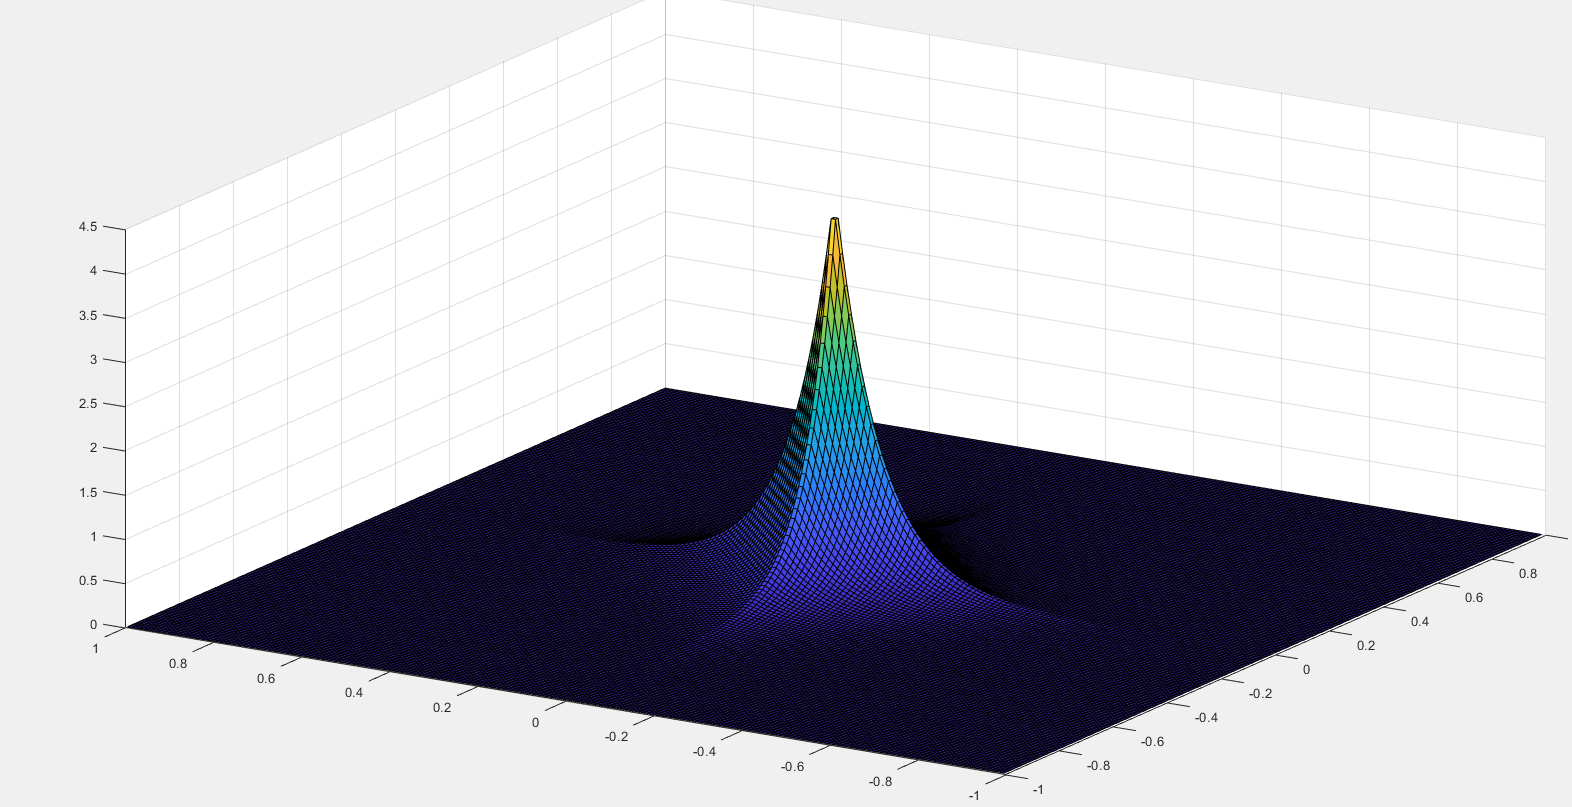
\includegraphics[width=15cm]{exp_protrusion}
\caption{Protrusion modelled with Exponential Decay}
\label{fig:exp_protrusion}
\end{figure}

A visualization is provided in Figure \ref{fig:exp_protrusion}. We utilize the following properties from Barret O'Neill (todo, cite here):

\begin{gather}
	E = \mathbf{r}_U \cdot \mathbf{r}_U \\
	F = \mathbf{r}_U \cdot \mathbf{r}_V \\
	G = \mathbf{r}_V \cdot \mathbf{r}_V \\
	EG - F^2 = ||\mathbf{r}_U \times \mathbf{r}_V||^2 \\
	L = S(\mathbf{r}_U) \cdot \mathbf{r}_U \\
	M = S(\mathbf{r}_U) \cdot \mathbf{r}_V = S(\mathbf{r}_V) \cdot \mathbf{r}_U \\
	N = S(\mathbf{r}_V) \cdot \mathbf{r}_V \\
	H = \frac{GL + EN - 2FM}{2(EG - F^2)}
\end{gather}

where H is the mean curvature, E, F, and G are the coefficients from the first fundamental form, and L, M, and N are the coefficients from the second fundamental form. The shape operator is defined as:

\begin{gather}
	S(\mathbf{V}) = -\nabla_{\mathbf{V}} \mathbf{U}
\end{gather}

where $\nabla_{V}$ is the covariant derivative with respect to a tangent vector $\mathbf{V}$, and $\mathbf{U}$ is the unit normal vector, which is given by:

\begin{gather}
	\mathbf{U} = \frac{\mathbf{r}_U \times \mathbf{r}_V}{||\mathbf{r}_U \times \mathbf{r}_V||}
\end{gather}

For our specific mapping $\mathbf{r}$, we obtain:

\begin{gather}
	E = 1 + \lambda^{2} e^{-2\lambda(U + V)} \\
	F = \lambda^{2} e^{-2\lambda(U + V)} \\
	G = 1 + \lambda^{2} e^{-2\lambda(U + V)} \\
	EG - F^{2} = 1 + 2\lambda^{2} e^{-2\lambda(U + V)} \\
	\mathbf{U} = \frac{\lambda e^{-\lambda(U + V)}(\mathbf{U}_1 + \mathbf{U}_2) + \mathbf{U}_3}{\sqrt{1 + 2\lambda^{2} e^{-2\lambda(U + V)}}}
\end{gather}

To calculate the coefficients of the second fundamental form, we begin by calculating the shape operator:

\begin{gather}
	S(\mathbf{r}_U) = -\nabla_{\mathbf{U}_1 - \lambda e^{\lambda(U + V)}\mathbf{U}_3} \frac{\lambda e^{-\lambda(U + V)}(\mathbf{U}_1 + \mathbf{U}_2) + \mathbf{U}_3}{\sqrt{1 + 2\lambda^{2} e^{-2\lambda(U + V)}}} \\
	= -\nabla_{\mathbf{U}_1} \frac{\lambda e^{-\lambda(U + V)}(\mathbf{U}_1 + \mathbf{U}_2) + \mathbf{U}_3}{\sqrt{1 + 2\lambda^{2} e^{-2\lambda(U + V)}}}
\end{gather}

The above reduction happens because there is no Z variable in the unit normal vector. Furthermore, a covariant derivative with respect to $\mathbf{U}_1$ is just a partial derivative with respect to $U$.

\begin{gather}
	S(\mathbf{r}_U) = -\frac{\partial}{\partial U} \frac{\lambda e^{-\lambda(U + V)}(\mathbf{U}_1 + \mathbf{U}_2) + \mathbf{U}_3}{\sqrt{1 + 2\lambda^{2} e^{-2\lambda(U + V)}}} \\
	= -\frac{\big(-\lambda^{2}(1 + 2\lambda^{2}e^{-2\lambda(U+V)})e^{-\lambda(U+V)} + 2\lambda^{4}e^{-3\lambda(U+V)}\big)(\mathbf{U}_1 + \mathbf{U}_2) + 2\lambda^{3}e^{-2\lambda(U+V)}\mathbf{U}_3}{(1 + 2\lambda^{2}e^{-2\lambda(U + V)})^{\frac{3}{2}}}
\end{gather}

Note that $S(\mathbf{r}_U) = S(\mathbf{r}_V)$ due to the symmetry of the above derivation. Furthermore, we observe $L = M = N$ once again due to symmetry. Thus:

\begin{gather}
	L = M = N = \frac{\lambda^{2}}{\sqrt{1 + 2\lambda^{2}e^{-2\lambda(U + V)}}}
\end{gather}

Finally, we derive an expression for the mean curvature.

\begin{gather}
	H = \frac{\lambda^{2}}{(1 + 2\lambda^{2}e^{-2\lambda(U + V)})^{\frac{3}{2}}}
\end{gather}

When $\lambda = 1$ the histogram of H as a random variable (estimated with Monte-Carlo), resembles Figure \ref{fig:exp_decay_distribution}.

\begin{figure}
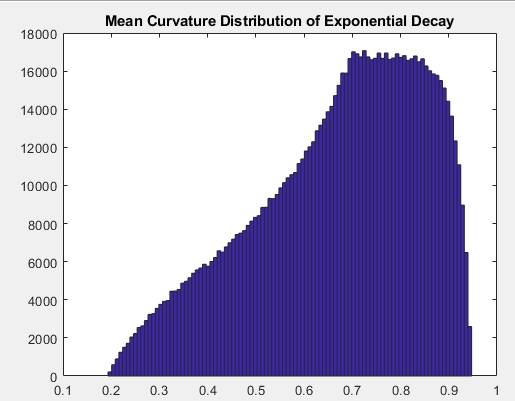
\includegraphics[width=15cm]{exp_decay_distribution}
\caption{Histogram of Mean Curvature with Exponential Decay}
\label{fig:exp_decay_distribution}
\end{figure}

\section{Mean Curvature Distribution Derivation (Gaussian Decay Case)}

We now wish to extend the previous derivation to protrusions with thinner tails and mass held closer to their centers.

\begin{gather}
	U, V iid \sim U(0,1) \\	
	Z = e^{-\lambda(U^2 + V^2)} \\
	\mathbf{r} = U \mathbf{U}_1 + V \mathbf{U}_2 + Z \mathbf{U}_3 \\
	\mathbf{r}_U = \mathbf{U}_1 - 2\lambda U e^{-\lambda(U^2 + V^2)}\mathbf{U}_3 \\
	\mathbf{r}_V = \mathbf{U}_2 - 2\lambda V e^{-\lambda(U^2 + V^2)}\mathbf{U}_3
\end{gather}

\begin{figure}
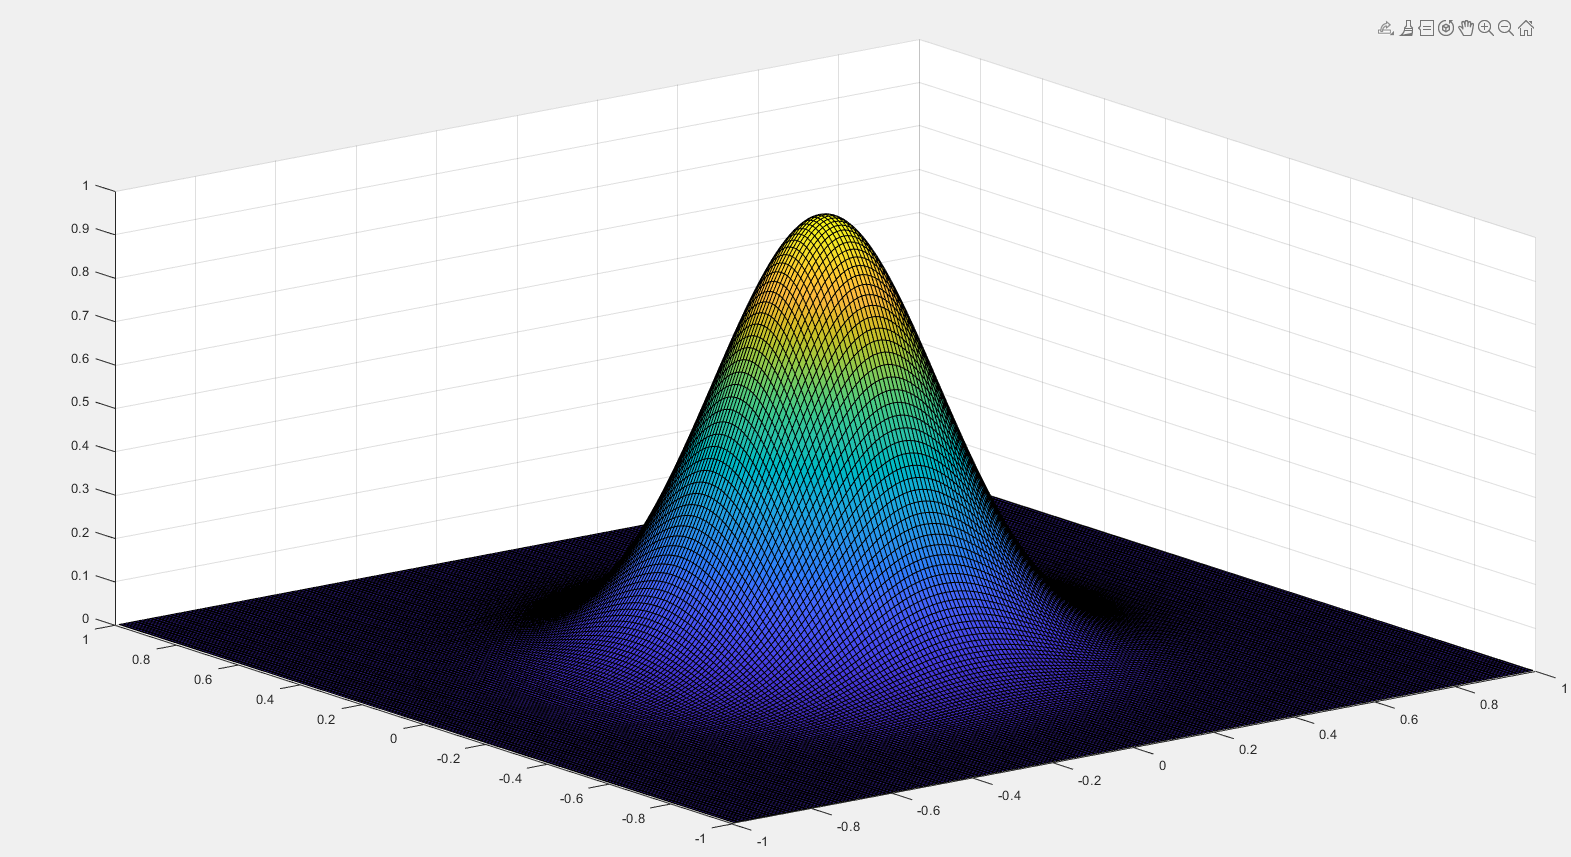
\includegraphics[width=15cm]{gaussian_protrusion}
\caption{Protrusion modelled with Gaussian Decay}
\label{fig:gaussian_protrusion}
\end{figure}

A visualization is provided in Figure \ref{fig:gaussian_protrusion}. For our new mapping $\mathbf{r}$, we obtain:

\begin{gather}
	E = 1 + 4 \lambda^{2} U^{2} e^{-2\lambda(U^2 + V^2)} \\
	F = 4 \lambda^{2} U V e^{-2\lambda(U^2 + V^2)} \\
	G = 1 + 4 \lambda^{2} V^{2} e^{-2\lambda(U^2 + V^2)} \\
	EG - F^{2} = 1 + 4\lambda^{2} e^{-2\lambda(U^2 + V^2)}(U^2 + V^2) \\
	\mathbf{U} = \frac{2\lambda e^{-\lambda(U^2 + V^2)}(U\mathbf{U}_1 + V\mathbf{U}_2) + \mathbf{U}_3}{\sqrt{1 + 4\lambda^{2} e^{-2\lambda(U^2 + V^2)}(U^2 + V^2)}}
\end{gather}

To calculate the coefficients of the second fundamental form, we begin by calculating the shape operator:

\begin{gather}
	S(\mathbf{r}_U) = -\nabla_{\mathbf{U}_1 - 2\lambda U e^{-\lambda(U^2 + V^2)}\mathbf{U}_3} \frac{2\lambda e^{-\lambda(U^2 + V^2)}(U\mathbf{U}_1 + V\mathbf{U}_2) + \mathbf{U}_3}{\sqrt{1 + 4\lambda^{2} e^{-2\lambda(U^2 + V^2)}(U^2 + V^2)}} \\
\end{gather}

Once again, this covariant derivative reduces to a partial derivative with respect to $U$.

\begin{gather}
	S(\mathbf{r}_U) = -\frac{\partial}{\partial U} \frac{2\lambda e^{-\lambda(U^2 + V^2)}(U\mathbf{U}_1 + V\mathbf{U}_2) + \mathbf{U}_3}{\sqrt{1 + 4\lambda^{2} e^{-2\lambda(U^2 + V^2)}(U^2 + V^2)}}
\end{gather}

Due to the complexity of the answer, $S(\mathbf{r}_U)$ is presented component by component:

\begin{gather}
	-\frac{2\lambda (1 - 2\lambda U^{2}) e^{-\lambda(U^2 + V^2)}\big(1 + 4\lambda^{2}e^{-2\lambda (U^2 + V^2)}(U^2 + V^2)\big) + 8\lambda^{3}U^{2}e^{-3\lambda(U^2 + V^2)}(1-2\lambda(U^2 + V^2))}{(1 + 4\lambda^{2} e^{-2\lambda(U^2 + V^2)}(U^2 + V^2))^{\frac{3}{2}}} \\
	-\frac{-4\lambda^{2} U V e^{-\lambda(U^2 + V^2)}\big(1 + 4\lambda^{2}e^{-2\lambda (U^2 + V^2)}(U^2 + V^2)\big) + 8\lambda^{3}U V e^{-3\lambda(U^2 + V^2)}(1-2\lambda(U^2 + V^2))}{(1 + 4\lambda^{2} e^{-2\lambda(U^2 + V^2)}(U^2 + V^2))^{\frac{3}{2}}}	\\
	\frac{4\lambda^{2}U e^{-2\lambda(U^2 + V^2)}(1 - 2\lambda(U^2 + V^2))}{(1 + 4\lambda^{2} e^{-2\lambda(U^2 + V^2)}(U^2 + V^2))^{\frac{3}{2}}}
\end{gather}

To reduce the complexity of this problem, for large enough $\lambda$, we assume that $e^{-3\lambda(U^2 + V^2)} \to 0$, as this takes a relatively small number to the third power. Thus:

\begin{gather}
	S(\mathbf{r}_U) \approx \frac{-2\lambda (1 - 2\lambda U^{2}) e^{-\lambda(U^2 + V^2)}}{\sqrt{1 + 4\lambda^{2} e^{-2\lambda(U^2 + V^2)}(U^2 + V^2)}}\mathbf{U}_1 + \\
	\frac{4\lambda^{2} U V e^{-\lambda(U^2 + V^2)}}{\sqrt{1 + 4\lambda^{2} e^{-2\lambda(U^2 + V^2)}(U^2 + V^2)}}\mathbf{U}_2 + \\
	\frac{4\lambda^{2}U e^{-2\lambda(U^2 + V^2)}(1 - 2\lambda(U^2 + V^2))}{(1 + 4\lambda^{2} e^{-2\lambda(U^2 + V^2)}(U^2 + V^2))^{\frac{3}{2}}}\mathbf{U}_3
\end{gather}

Once again utilizing $e^{-3\lambda(U^2 + V^2)} \to 0$, and the symmetry of $S(\mathbf{r}_U)$ and $S(\mathbf{r}_V)$:

\begin{gather}
	L = S(\mathbf{r}_U) \cdot \mathbf{r}_U \approx \frac{-2\lambda (1 - 2\lambda U^{2}) e^{-\lambda(U^2 + V^2)}}{\sqrt{1 + 4\lambda^{2} e^{-2\lambda(U^2 + V^2)}(U^2 + V^2)}} \\
	M = S(\mathbf{r}_U) \cdot \mathbf{r}_V \approx \frac{4\lambda^{2} U V e^{-\lambda(U^2 + V^2)}}{\sqrt{1 + 4\lambda^{2} e^{-2\lambda(U^2 + V^2)}(U^2 + V^2)}} \\
	N = S(\mathbf{r}_V) \cdot \mathbf{r}_V \approx \frac{-2\lambda (1 - 2\lambda V^{2}) e^{-\lambda(U^2 + V^2)}}{\sqrt{1 + 4\lambda^{2} e^{-2\lambda(U^2 + V^2)}(U^2 + V^2)}} \\
\end{gather}

Finally, (applying $e^{-3\lambda(U^2 + V^2)} \to 0$ once more), we obtain:

\begin{gather}
	H = \frac{2\big(\lambda(U^2 + V^2) - 1 \big)e^{-\lambda(U^2 + V^2)}}{(1 + 4\lambda^{2} e^{-2\lambda(U^2 + V^2)}(U^2 + V^2))^{\frac{3}{2}}}
\end{gather}

When $\lambda = 1$ the histogram of H as a random variable (estimated with Monte-Carlo), resembles Figure \ref{fig:gaussian_decay_distribution}.

\begin{figure}
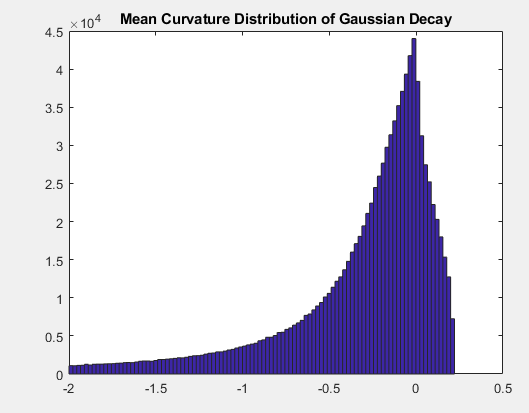
\includegraphics[width=15cm]{gaussian_decay_distribution}
\caption{Histogram of Mean Curvature with Exponential Decay}
\label{fig:gaussian_decay_distribution}
\end{figure}

%% The Appendices part is started with the command \appendix;
%% appendix sections are then done as normal sections
%% \appendix

%% \section{}
%% \label{}

%% References
%%
%% Following citation commands can be used in the body text:
%% Usage of \cite is as follows:
%%   \cite{key}         ==>>  [#]
%%   \cite[chap. 2]{key} ==>> [#, chap. 2]
%%

%% References with bibTeX database:

\bibliographystyle{elsarticle-num}
\bibliography{<your-bib-database>}

%% Authors are advised to submit their bibtex database files. They are
%% requested to list a bibtex style file in the manuscript if they do
%% not want to use elsarticle-num.bst.

%% References without bibTeX database:

% \begin{thebibliography}{00}

%% \bibitem must have the following form:
%%   \bibitem{key}...
%%

% \bibitem{}

% \end{thebibliography}


\end{document}

%%
%% End of file 